\documentclass[margin=0.5cm]{standalone}

\usepackage{tikz}
\usepackage{xcolor}

\usetikzlibrary{arrows.meta}


\begin{document}

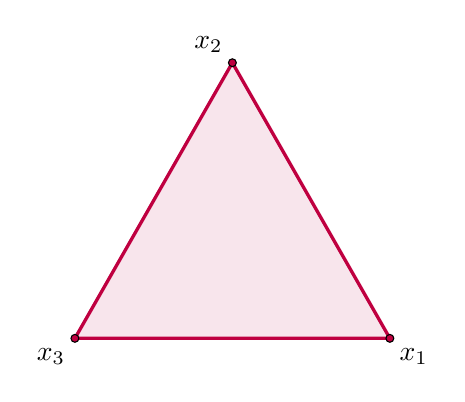
\begin{tikzpicture}
  \draw[purple, very thick, fill=purple, fill opacity=0.1] (0,0) -- (2, 3.5) -- (4,0) -- (0,0);

  \draw[fill=purple] (2.0,3.5) circle[radius=0.05];
  \draw (2.0,3.5) node[anchor=south east] {$x_2$};
  \draw[fill=purple] (4,0) circle[radius=0.05];
  \draw (4,0) node[anchor=north west] {$x_1$};
  \draw[fill=purple] (0,0) circle[radius=0.05];
  \draw (0,0) node[anchor=north east] {$x_3$};
\end{tikzpicture} 

\end{document}
